\documentclass[pdf,12pt]{beamer}

\usepackage{../esslli}

\title{Numeral Semantics {\normalfont | Monday}}
\author{Lisa Bylinina \& Rick Nouwen}
\date{ESSLLI 2019}
\usepackage{qtree}


\begin{document}

\begin{frame}\titlepage\end{frame}

\begin{frame}{Numeral Semantics}

\note{This is where we say the abstract. This is also the point where we might (or might not) ask the students about their background / interests.}
  
  \vfill
  \begin{center}
{ \huge $\sem{\mbox{\l{twelve}}}$}
\pause
\vfill
{\Large $\sem{\mbox{\l{Twelve students came to the party}}}$}
\end{center}\vfill
  
\end{frame}

\begin{frame}{Overview}
\begin{itemize}
\item[] \textbf{Monday}: Theories of numeral semantics
\item[] \textbf{Tuesday}: Continued
\item[] \textbf{Wednesday}: Continued \\[1em]
\item[] \textbf{Thursday}: (Im)precision \\[1em]
\item[] \textbf{Friday}: Beyond semantics
\end{itemize}
\end{frame}


\begin{frame}{Numerals as determiners}

\begin{minipage}{.75\textwidth}
\begin{flushright}

  \l{{\bf Twelve} students came to the party.}

  \pause

  \l{{\bf Several} students came to the party.}

  \l{{\bf Some} students came to the party.}

  \l{{\bf Most} students came to the party.}

  \l{{\bf No} students came to the party.}

\end{flushright}
\end{minipage}

 \end{frame}

\begin{frame}[t]{Generalized Quantifier Theory}
%\vspace*{-2em}

\note{clean up slide}
\small{
\only<1>{\Tree [.{\l{Q student(s) came to the party}} [ Q [.A student(s) ] ] \qroof{came to the party}.{B} ]}

\only<2->{\Tree [.{\l{Q student(s) came to the party}} [.{$\langle e, t \rangle, t \rangle$} {Q \\ $\langle \langle e,t \rangle, \langle \langle e, t \rangle, t \rangle \rangle$} [.{A \\ $\langle e,t \rangle $} student(s) ] ] \qroof{came to the party}.{B \\ $\langle e,t \rangle $} ]}

\vspace*{1em}
\only<3>{
  every(A)(B) iff A$\subseteq$B\\
  no(A)(B) iff A$\cap$B=$\emptyset$\\
  some(A)(B) iff A$\cap$B$\not=\emptyset$
}}

\only<4>{    {\bf Big research question:} Which quantifiers are realised in NL?
 What properties do all realised quantifiers share?
}

\vfill \hfill
 \only<2->{\fn{Barwise \& Cooper, 1980; Keenan \& Stavi 1984}}

  \end{frame}

  
 \begin{frame}{Constraints on quantifiers}

\note{clean up slide} 
    
%    \footnote{\fn{van Benthem, 1984}}
    
%    {\sc cons}: $Q(A)(B) \Leftrightarrow Q(A)(A\cap B)$

For any bijection $F$: \\
    {\sc quant}: $Q(A)(B) \Leftrightarrow Q(F(A))(F(B))$ \hfill \fn{van Benthem, 1984}

    \pause

Upshot: Only cardinalities matter

\begin{center}
\begin{tabular}{rcl}
  every(A)(B) & iff & $|$A$\cap$B$|$=$|$A$|$\\
  no(A)(B) & iff & $|$A$\cap$B$|$=0\\
  some(A)(B) & iff & $|$A$\cap$B$|\not=$0\\ \pause
  & & \\
  twelve(A)(B) & iff & $|$A$\cap$ B$|$=12 \\
\end{tabular}
\end{center}

    \end{frame}

\begin{frame}{Numerals are not quantifiers}
  \pause

  (1) \l{{\bf Twelve} students came to the party}

  (2) \l{{\bf Twelve} people can fit in the lift}
  
\pause 

(2') \l{{\bf Most} people can fit in the lift}

  \note{point to make: if we impose GQ to (2) we look at the set of atomic(!) people who can fit in the lift and we count them. Tis is not what the sentenc emeans. Rather, we want to look at groups of twleve people and say that they generally have this property..
When i ntrouble, we could compare (2) to ``most students can fit in the lift''
}

\pause

(3) \l{Every {\bf two} houses come with one parking space.}
  
\end{frame}

\begin{frame}{Numerals are not quantifiers}

  (4) \l{Rod A is {\bf three} times longer than rod B.}

\note{The most natural way of looking at this example does not involve cardinality. Take a length and multiply it by 3. }
  
  (5) \l{{\bf Two} is a Fibonacci number.}

  \note{Duh, there's nothing to intersect}
 

\note{At this point we should introduce the thought that there's maths and there are words that we use to talk about maths. What is the rleation between the realm of arithmetic and NL? These examples suggest that sometimes arithmetic aspects to numbers end up in natural language}

  \end{frame}


  \begin{frame}{Three strands of thought}

    1. the number view

    $\sem{\mbox{\l{twelve}}}\ =\ 12$\vfill

    2. the modifier view

    $\sem{\mbox{\l{twelve}}}\ =\ \lambda x.\#x=12$\vfill

    3. the quantifier view (revisited)

    $\sem{\mbox{\l{twelve}}}\ =\ $ the set of intervals that end in 12
    
\end{frame}

\begin{frame}[t]{The number view}

  $\sem{\mbox{\l{twelve}}}\ =\ 12$ \qquad whatever that means

  \vfill

  \only<2>{
  (5) \l{{\bf Two} is a Fibonacci number.}

  $\sem{\mbox{is a Fibonacci number}}$ = $\{0,1,2,3,5,8,13,21,34,\ldots \}$}

\only<3>{

  (4') \l{Rod A is longer than rod B.}

  means: the length of rod A $>$ the length of rod B
  
  (4) \l{Rod A is {\bf three} times longer than rod B.}

  means: the length of rod A = 3 $\times$ the length of rod B


  \note{In these examples, we do not really need to know what a number is. Whatever it is, it does what is does elsewhere.
  But what is then the relation between numbers and numerals expressing set cardinality.}

}

  
  \end{frame}

  \begin{frame}{What could a number be?}

    Basic semantic ontology: 
    \begin{itemize}
    \item Entities; type $e$
    \item Truth-values; type $t$
    \end{itemize}
\pause
\vfill
We are going to add {\bf degrees} to this picture: type $d$

\begin{itemize}
\item Degrees are like entities, but ordered
\end{itemize}
\vspace{-1ex}
\begin{center} John $<$ Mary \qquad $2 < 3$ \end{center}
\vspace{-1ex}
\begin{itemize}
\item Numbers are a special case of degrees
\end{itemize}
  
  \end{frame}

  \begin{frame}{What could a degree be?}

    (6) \l{John is taller than Mary} \pause \\
    John's height $>$ Mary's height
    
    \vfill \pause
    
    (7) \l{John is 2cm taller than Mary} \pause \\
    John's height = Mary's height + 2cm
 
 \vfill \pause
 
    (8) \l{John is this tall} \pause \\
    \l{this} demonstrates a degree

  \end{frame}


  \begin{frame}{What could a degree be?}

\begin{itemize}
\item \hspace*{-1em} We seem to be committed to a domain of abstract entities
\item \hspace*{-1em}  We don't have to be: 
\begin{itemize}
\item \hspace*{-1.5em} Cresswell 1977: \l{tall} involves an ability to decide that $j$ $<$ $m$
\item \hspace*{-1.5em} We can see degrees as equivalence classes of individuals 
\end{itemize}
\end{itemize}
  
\begin{center}
 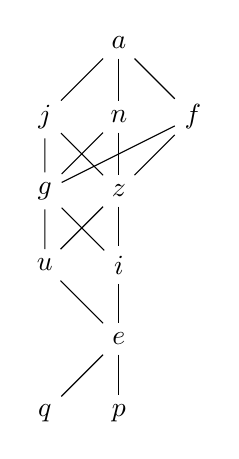
\begin{tikzpicture}[scale=.47]

%\clip(-3,-6) rectangle (6,12);
  \node (n1) at (0,5) {$a$};
  \node (n21) at (-2,3) {$j$};
  \node (n22) at (0,3) {$n$};
  \node (n23) at (2,3) {$f$};
  \node (n31) at (-2,1) {$g$};
  \node (n32) at (0,1) {$z$};
  \node (n41) at (-2,-1) {$u$};
  \node (n42) at (0,-1) {$i$};
  \node (n51) at (0,-3) {$e$};
  \node (n61) at (-2,-5) {$q$};
  \node (n62) at (0,-5) {$p$};
  \draw (n1) -- (n21);
  \draw (n1) -- (n22);
  \draw (n1) -- (n23);
  \draw (n21) -- (n31);
  \draw (n21) -- (n32);
  \draw (n22) -- (n31);
  \draw (n22) -- (n32);
  \draw (n23) -- (n31);
  \draw (n23) -- (n32);
  \draw (n31) -- (n41);
  \draw (n31) -- (n42);
  \draw (n32) -- (n41);
  \draw (n32) -- (n42);
  \draw (n41) -- (n51);
  \draw (n42) -- (n51);
  \draw (n51) -- (n61);
  \draw (n51) -- (n62);
 \end{tikzpicture}
\end{center} 
  
    \end{frame}

\begin{frame}{Would could a degree be?}
\begin{columns}
\begin{column}{.25\textwidth}
 \begin{tikzpicture}[scale=.47]

\clip(-3,-6) rectangle (6,9);
  \node (n1) at (0,5) {$a$};
  \node (n21) at (-2,3) {$j$};
  \node (n22) at (0,3) {$n$};
  \node (n23) at (2,3) {$f$};
  \node (n31) at (-2,1) {$g$};
  \node (n32) at (0,1) {$z$};
  \node (n41) at (-2,-1) {$u$};
  \node (n42) at (0,-1) {$i$};
  \node (n51) at (0,-3) {$e$};
  \node (n61) at (-2,-5) {$q$};
  \node (n62) at (0,-5) {$p$};
  \draw (n1) -- (n21);
  \draw (n1) -- (n22);
  \draw (n1) -- (n23);
  \draw (n21) -- (n31);
  \draw (n21) -- (n32);
  \draw (n22) -- (n31);
  \draw (n22) -- (n32);
  \draw (n23) -- (n31);
  \draw (n23) -- (n32);
  \draw (n31) -- (n41);
  \draw (n31) -- (n42);
  \draw (n32) -- (n41);
  \draw (n32) -- (n42);
  \draw (n41) -- (n51);
  \draw (n42) -- (n51);
  \draw (n51) -- (n61);
  \draw (n51) -- (n62);
 \end{tikzpicture}

\end{column}

\begin{column}{.75\textwidth}
\begin{itemize}
\item \hspace*{-1.5em} This is an ordinal scale 
\item \hspace*{-1.5em} No distances, no zero, no multiplication
\item \hspace*{-1.5em} To make this work, height etc. would need to be added to the equivalence classes \fn{(Bale 2011)}
\item \hspace*{-1.5em} Back to square one 
\end{itemize}

\end{column}
\end{columns}



    \note{
    
        multiplicative will need a ratio scale however so we need to do some work; basically we would need to introduce operations on classes, in particular addition. this makes clear again that degrees (whatever they are) are dependent on the kind of operations that we know exist for numbers.

upshot: we will need to assume more than just entities anyway

  - Numbers are ordered, this distinguishes this domain from the domain of entities

  - Related: degree constructions in Natural language. There is the assumption that degrees exist because we need something to explain the expression of comparison and intensity.

  - Even if you believe degrees are necessary, the ontological commitment is not necessarily so large, since you could see degrees as a short-cut for a bigger structure.

  - do cresswell and bale

  - what they do is what frege did earlier
 } 
  

\end{frame}

\begin{frame}{The number view: challenges}

  How does this meaning connect with nouns, to give us sets with particular cardinalities?

  (1) \l{Twelve students came to the party.}

  (9) \l{Twelve people can fit in the lift.}
  
  (10) \l{Every two houses come with one parking space.}


  \pause \vfill

  {\bf Preview of options:}
\begin{enumerate}
\item  Keep this meaning of numerals, add something that connects it with nouns (lecture 2)
\item Assume a different meaning of numerals (in this position)
\end{enumerate}    
   
\end{frame}


    \begin{frame}[t]{The modifier view}
      \pause
\vspace*{4ex}

      $\sem{\mbox{twelve}}$ = $\lambda x.\#x=12$ \hfill (the set of groups of cardinality 12)

      $\sem{\mbox{American}}$ = $\lambda x.american(x)$ \hfill (the set of American entities)

\vspace*{4ex}
      \only<2>{      \Tree [. [.$\lambda x.american(x)$ American ] [.$\lambda x.student(x)$ student ] ]}

      \only<3>{      \Tree [.$\lambda x.american(x)\land student(x)$ [.$\lambda x.american(x)$ American ] [.$\lambda x.student(x)$ student ] ]}

      \only<4>{      \Tree [. [.$\lambda x.\#x=12$ twelve ] [.$\lambda x.^*student(x)$ students ] ]}

            \only<5>{      \Tree [.$\lambda x.\#x=12\land ^*student(x)$ [.$\lambda x.\#x=12$ twelve ] [.$\lambda x.^*student(x)$ students ] ]}


            \only<6->{\begin{center}\l{every twelve students} now parallels \l{every American student}\end{center}} \only<7>{\begin{center}  The numeral expresses cardinality, not quantificational force\end{center} }

            
            
      \end{frame}

      \begin{frame}{The modifier view}

In the absence of a determiner, it's parallel to a bare plural:

        (1) \l{Twelve students came to the party}

        (11) \l{American students came to the party}
        
      \pause \vfill We will return to this.  
        
      \end{frame}

      \begin{frame}[t]{The modifier view: challenges}

        \pause

        (5) \l{{\bf Two} is a Fibonacci number} \pause

        This is not NP ellipsis:

        (5') *\l{{\bf Two} are a fibonacci number}

        (5'') \l{{\bf Two} boxes are/*is open} 

      \pause
\vfill 
Maybe it's not a problem: 

\vfill

        $\sem{\mbox{\l{is a Fibonacci number}}}$ = \\$\{\lambda x.\#x=1,\ \lambda x.\#x=2,\ \lambda x.\#x=3, \lambda x.\#x=5,\ldots\}$

\vfill
    
      
      \end{frame}

\begin{frame}[fragile]{Type landscape}

 \hspace*{-2em}   \begin{tikzpicture}[every node/.style={anchor=base,align=center,text height=4ex,text width=2cm}]
  \matrix[matrix of nodes,nodes={draw,
    draw,inner sep=8pt,minimum height=3.1ex},
    column sep=2ex,row sep=1.2ex,inner sep=2ex,
    rounded corners]  {
  {$e$\\ {\scriptsize entity}} & {$\langle e,t\rangle$\\ {\scriptsize property}} & {$\langle \langle e,t\rangle, t\rangle$\\ {\scriptsize quantifier}} & |[fill=green!30]|{{\scriptsize $\langle \langle e,t \rangle, \langle \langle e,t\rangle, t\rangle \rangle$} \\ {\scriptsize quantifier}}\\
  {$d$\\ {\scriptsize degree}} & {$\langle d,t\rangle$\\ {\scriptsize degree property}} & {$\langle \langle d,t\rangle, t\rangle$\\ {\scriptsize \mbox{degree quantifier}}} & \\
 };

\end{tikzpicture}
\end{frame}

\begin{frame}[fragile]{Type landscape}

 \hspace*{-2em}   \begin{tikzpicture}[every node/.style={anchor=base,align=center,text height=4ex,text width=2cm}]
  \matrix[matrix of nodes,nodes={draw,
    draw,inner sep=8pt,minimum height=3.1ex},
    column sep=2ex,row sep=1.2ex,inner sep=2ex,
    rounded corners]  {
  {$e$\\ {\scriptsize entity}} & {$\langle e,t\rangle$\\ {\scriptsize property}} & {$\langle \langle e,t\rangle, t\rangle$\\ {\scriptsize quantifier}} & |[fill=gray!30]|{{\scriptsize $\langle \langle e,t \rangle, \langle \langle e,t\rangle, t\rangle \rangle$} \\ {\scriptsize quantifier}}\\
  |[fill=green!30]|{$d$\\ {\scriptsize degree}} & {$\langle d,t\rangle$\\ {\scriptsize degree property}} & {$\langle \langle d,t\rangle, t\rangle$\\ {\scriptsize \mbox{degree quantifier}}} & \\
 };

\end{tikzpicture}
\end{frame}

\begin{frame}[fragile]{Type landscape}

 \hspace*{-2em}   \begin{tikzpicture}[every node/.style={anchor=base,align=center,text height=4ex,text width=2cm}]
  \matrix[matrix of nodes,nodes={draw,
    draw,inner sep=8pt,minimum height=3.1ex},
    column sep=2ex,row sep=1.2ex,inner sep=2ex,
    rounded corners]  {
  {$e$\\ {\scriptsize entity}} & |[fill=green!30]|{$\langle e,t\rangle$\\ {\scriptsize property}} & {$\langle \langle e,t\rangle, t\rangle$\\ {\scriptsize quantifier}} & |[fill=gray!30]|{{\scriptsize $\langle \langle e,t \rangle, \langle \langle e,t\rangle, t\rangle \rangle$} \\ {\scriptsize quantifier}}\\
  |[fill=gray!30]|{$d$\\ {\scriptsize degree}} & {$\langle d,t\rangle$\\ {\scriptsize degree property}} & {$\langle \langle d,t\rangle, t\rangle$\\ {\scriptsize \mbox{degree quantifier}}} & \\
 };

\end{tikzpicture}
\end{frame}

\begin{frame}[fragile]{Type landscape}

 \hspace*{-2em}   \begin{tikzpicture}[every node/.style={anchor=base,align=center,text height=4ex,text width=2cm}]
  \matrix[matrix of nodes,nodes={draw,
    draw,inner sep=8pt,minimum height=3.1ex},
    column sep=2ex,row sep=1.2ex,inner sep=2ex,
    rounded corners]  {
  {$e$\\ {\scriptsize entity}} & |[fill=gray!30]|{$\langle e,t\rangle$\\ {\scriptsize property}} & {$\langle \langle e,t\rangle, t\rangle$\\ {\scriptsize quantifier}} & |[fill=gray!30]|{{\scriptsize $\langle \langle e,t \rangle, \langle \langle e,t\rangle, t\rangle \rangle$} \\ {\scriptsize quantifier}}\\
  |[fill=gray!30]|{$d$\\ {\scriptsize degree}} & {$\langle d,t\rangle$\\ {\scriptsize degree property}} & |[fill=green!30]|{$\langle \langle d,t\rangle, t\rangle$\\ {\scriptsize \mbox{degree quantifier}}} & \\
 };

\end{tikzpicture}
\end{frame}

\begin{frame}[fragile]{Type landscape}

 \hspace*{-2em}   \begin{tikzpicture}[every node/.style={anchor=base,align=center,text height=4ex,text width=2cm}]
  \matrix[matrix of nodes,nodes={draw,
    draw,inner sep=8pt,minimum height=3.1ex},
    column sep=2ex,row sep=1.2ex,inner sep=2ex,
    rounded corners]  {
  {$e$\\ {\scriptsize entity}} & |[fill=gray!30]|{$\langle e,t\rangle$\\ {\scriptsize property}} & {$\langle \langle e,t\rangle, t\rangle$\\ {\scriptsize quantifier}} & |[fill=gray!30]|{{\scriptsize $\langle \langle e,t \rangle, \langle \langle e,t\rangle, t\rangle \rangle$} \\ {\scriptsize quantifier}}\\
  |[fill=gray!30]|{$d$\\ {\scriptsize degree}} & {$\langle d,t\rangle$\\ {\scriptsize degree property}} & |[fill=gray!30]|{$\langle \langle d,t\rangle, t\rangle$\\ {\scriptsize \mbox{degree quantifier}}} & \\
 };

\end{tikzpicture}
\end{frame}

\begin{frame}[plain]{}
\begin{center}{\Huge See you tomorrow!}\end{center}
\end{frame}
        
\end{document}